\chapter{Understanding Systematic Reviews} \label{chap:sysrev}

This chapter provides a foundational understanding of systematic reviews, their methodological framework, and best practices that \texttt{prismAId} is designed to support.

\section{What is a Systematic Review?}

A systematic review is a rigorous, transparent approach to synthesizing existing research literature on a specific research question.\tip{The term "systematic" emphasizes that these reviews follow an explicit, reproducible methodology.} Unlike narrative reviews, which offer subjective summaries of selected studies, systematic reviews aim to identify, evaluate, and integrate findings from all relevant studies using predefined protocols.

Systematic reviews serve several critical purposes in scientific research:\note{Systematic reviews differ from other literature reviews in their methodological rigor, comprehensive search strategies, explicit inclusion criteria, and transparent reporting of methods.}

\begin{itemize}
    \item \textbf{Consolidating Knowledge}: They integrate findings across multiple studies, providing a comprehensive understanding of available evidence.
    \item \textbf{Identifying Gaps}: By mapping existing literature, they reveal knowledge gaps and research opportunities.
    \item \textbf{Minimizing Bias}: Their structured approach reduces subjective biases in literature selection and interpretation.
    \item \textbf{Supporting Evidence-Based Decisions}: They provide synthesized evidence to inform policy, practice, and further research.
\end{itemize}

Systematic reviews can also include meta-analyses, which statistically combine results from multiple studies to estimate overall effects.\warning{Meta-analyses require statistical expertise and should only be conducted when studies are sufficiently similar in design and outcome measures.}

\section{Key Concepts \& Methodology}

The systematic review process follows a well-established methodology that ensures transparency and reproducibility. The widely adopted PRISMA framework (Preferred Reporting Items for Systematic Reviews and Meta-Analyses) outlines the following essential steps:

\begin{infobox}[PRISMA 2020 Framework Overview]
\begin{lstlisting}
PRISMA 2020 Key Components:
1. Title & Abstract
2. Introduction (Rationale, Objectives)
3. Methods (Eligibility criteria, Information sources, Search strategy,
   Selection process, Data extraction, Study quality assessment)
4. Results (Study selection, Study characteristics, Risk of bias,
   Results of syntheses, Reporting biases)
5. Discussion (Summary, Limitations, Conclusions)
6. Other information (Registration, Protocol, Support)

Full checklist available at: prisma-statement.org
\end{lstlisting}
\end{infobox}

\subsection{Pre-Review Planning}

Before beginning the review, researchers must:\tip{Well-formulated research questions are specific, clear, and focused. Avoid questions that are too broad ("What is known about climate change?") or too narrow ("What is the effect of a 1.5°C temperature increase on the reproduction of a specific butterfly species in northern Sweden?").}

\begin{itemize}
    \item \textbf{Formulate Research Questions}: Define specific, answerable questions using frameworks like PICO (Population, Intervention, Comparison, Outcome) or PEO (Population, Exposure, Outcome).
    \item \textbf{Develop Review Protocol}: Create a detailed plan specifying search strategies, inclusion/exclusion criteria, and analysis methods.\reminder{Always register your systematic review protocol before beginning the review process. This prevents bias and demonstrates methodological transparency.}

    \item \textbf{Register Protocol}: Pre-register the protocol in repositories like PROSPERO to enhance transparency and prevent duplication.
\end{itemize}

\begin{infobox}[PICO Framework Example]
\begin{lstlisting}
Research Question: "What is the effect of cognitive behavioral therapy compared to medication on depression symptoms in adults?"

P (Population): Adults with depression
I (Intervention): Cognitive behavioral therapy
C (Comparison): Medication treatment
O (Outcome): Depression symptom reduction
\end{lstlisting}
\end{infobox}

\subsection{Literature Search \& Selection}

The search and selection phase involves:

\begin{itemize}
    \item \textbf{Comprehensive Search}: Implement systematic search strategies across multiple databases using carefully constructed search terms.\warning{Relying on a single database significantly increases the risk of missing relevant studies. Research shows that even comprehensive databases like PubMed or Web of Science individually capture only 50-75\% of eligible studies in many fields.}
    \item \textbf{Screening}: Apply inclusion and exclusion criteria in a two-stage process: title/abstract screening followed by full-text assessment.\note{prismAId's Screening tool can automate the initial filtering of manuscripts using deduplication, language detection, article type classification, and topic relevance scoring, significantly reducing the manual workload before full-text download.}
    \item \textbf{PRISMA Flow Diagram}: Document the selection process, including numbers of studies identified, screened, assessed for eligibility, and included.
\end{itemize}

\begin{infobox}[PubMed Search Strategy Example]
\begin{lstlisting}
("climate change"[MeSH Terms] OR "global warming"[Title/Abstract])
AND
("agriculture"[MeSH Terms] OR "crop yield"[Title/Abstract] OR "food production"[Title/Abstract])
AND
("adaptation"[Title/Abstract] OR "mitigation"[Title/Abstract])
AND
("2010"[Date - Publication] : "2023"[Date - Publication])
\end{lstlisting}
\end{infobox}

\subsection{Data Extraction \& Quality Assessment}

Once relevant studies are identified, researchers:

\begin{itemize}
    \item \textbf{Extract Data}: Systematically collect relevant information from each study using standardized forms.\tip{Create your data extraction form in digital format (e.g., spreadsheet) rather than paper. This facilitates easier data manipulation, sharing among team members, and integration with analysis software.}
    \item \textbf{Assess Quality}: If a manual review, evaluate methodological rigor using tools like the Cochrane Risk of Bias Tool or GRADE (Grading of Recommendations Assessment, Development, and Evaluation). If AI-assisted, follow approaches described in this manual.
    \item \textbf{Document Uncertainties}: Record ambiguities or missing information, often contacting original authors for clarification.
\end{itemize}

\begin{infobox}[Data Extraction Template Example]
\begin{lstlisting}
Study ID: [Reference ID]
Citation: [Full citation in standard format]
Study Design: [RCT, cohort, case-control, etc.]
Population Characteristics:
  - Sample size: [n=]
  - Demographics: [age, gender, location, etc.]
  - Inclusion criteria: [as reported]
Intervention/Exposure:
  - Type: [specific details]
  - Duration: [time period]
  - Frequency: [how often applied]
Comparison/Control: [details of control group]
Outcomes:
  - Primary: [specific measure, unit]
  - Secondary: [additional measures]
Results:
  - Main findings: [effect sizes, p-values]
  - Subgroup analyses: [if applicable]
Study Quality Assessment:
  - Tool used: [e.g., Cochrane RoB, GRADE]
  - Overall rating: [Low/Moderate/High risk of bias]
  - Key limitations: [specific methodological concerns]
Notes: [Additional relevant information]
\end{lstlisting}
\end{infobox}

\subsection{Synthesis \& Analysis}

The final analytical phase includes:

\begin{itemize}
    \item \textbf{Narrative Synthesis}: Organize and summarize findings qualitatively, identifying patterns and relationships.
    \item \textbf{Quantitative Synthesis}: When appropriate, conduct meta-analysis to statistically combine results.\note{Not all systematic reviews are suitable for meta-analysis. When studies use different outcome measures or have high methodological heterogeneity, narrative synthesis may be more appropriate.}
    \item \textbf{Heterogeneity Assessment}: Evaluate variations in study designs, populations, and outcomes.
    \item \textbf{Subgroup Analysis}: Explore how findings vary across different study characteristics or populations.
\end{itemize}
\warning{Systematic reviews require significant time and resources. A comprehensive review typically takes 6-18 months to complete when conducted manually. Plan your timeline accordingly and consider the efficiency benefits tools like \texttt{prismAId} can provide.}
\begin{commandbox}[R Code Example for Forest Plot Creation]
\begin{lstlisting}[language=R]
# Basic R code for meta-analysis and forest plot
library(meta)

# Create meta-analysis object
meta_analysis <- metagen(TE = effect_size,
                         seTE = standard_error,
                         studlab = study_name,
                         data = extracted_data,
                         sm = "SMD")

# Generate forest plot
forest(meta_analysis,
       sortvar = year,
       prediction = TRUE,
       print.tau2 = TRUE,
       print.I2 = TRUE)
\end{lstlisting}
\end{commandbox}

\section{Best Practices}

Conducting high-quality systematic reviews involves adhering to several best practices:

\subsection{Transparency \& Reproducibility}

\begin{itemize}
    \item \textbf{Detailed Documentation}: Record all decisions, search strategies, and methods.\reminder{Document all exclusion decisions during screening. For transparency, maintain a list of studies excluded at the full-text review stage with specific reasons for exclusion.}
    \item \textbf{PRISMA Compliance}: Follow PRISMA guidelines for reporting.
    \item \textbf{Open Data}: When possible, share data extraction forms and analysis files.
\end{itemize}

\subsection{Methodological Rigor}

\begin{itemize}
    \item \textbf{Comprehensive Searching}: Use multiple databases and supplementary methods like citation tracking.
    \item \textbf{Dual Screening}: If a manual review, have at least two independent reviewers screen studies, with a third resolving disagreements.\tip{Again if you do not want to take advantage of prismAId and you are proceeding with a manual review, before full screening, conduct a calibration exercise where all reviewers independently screen the same 5-10 studies, then compare results to ensure consistent application of criteria. This identifies misunderstandings early and improves inter-rater reliability.}
    \item \textbf{Pilot Testing}: Test screening and data extraction procedures on a subset of studies.
\end{itemize}

\begin{infobox}[Screening Criteria Documentation]
\begin{lstlisting}
Inclusion Criteria:
- Population: Adults (18+) with Type 2 Diabetes
- Intervention: Digital health interventions
- Comparison: Standard care or other interventions
- Outcomes: HbA1c levels, quality of life measures
- Study Design: Randomized controlled trials
- Publication: Peer-reviewed, English language, 2010-2023

Exclusion Criteria:
- Studies focusing exclusively on Type 1 Diabetes
- Non-digital interventions
- Conference abstracts or proceedings
- Studies without control groups
\end{lstlisting}
\end{infobox}

\subsection{Managing Bias}

\begin{itemize}
    \item \textbf{Publication Bias}: Search for unpublished studies and conduct funnel plot analysis when applicable.\warning{Be cautious of language bias. Limiting searches to English-language publications can miss important evidence, particularly in fields with significant international research or regional focus.}

    \item \textbf{Selection Bias}: Use predefined, objective inclusion criteria.
    \item \textbf{Confirmation Bias}: If a manual review, have team members with diverse perspectives review the evidence.
\end{itemize}

\begin{commandbox}[Code for Publication Bias Assessment]
\begin{lstlisting}[language=R]
# Funnel plot and Egger's test in R
library(meta)

# Create funnel plot
funnel(meta_analysis,
       studlab = TRUE,
       contour = TRUE)

# Perform Egger's test for publication bias
metabias(meta_analysis, method = "linreg")
\end{lstlisting}
\end{commandbox}

\subsection{Team Collaboration}

\begin{itemize}
    \item \textbf{Multidisciplinary Teams}: Ideally, include subject matter experts, methodologists, and librarians.\note{Consulting with a research librarian can significantly improve search strategy quality. Their expertise in database syntax and controlled vocabulary (e.g., MeSH terms) helps ensure comprehensive literature identification.}\reminder{The most robust manual systematic reviews often involve teams rather than individual researchers. If working alone, consider consulting with colleagues at critical decision points to reduce subjectivity and to take advantage of prismAId.}
    \item \textbf{Regular Calibration}: Conduct ongoing discussions to ensure consistent application of criteria.
    \item \textbf{Clear Roles}: If there is a team, define responsibilities for each team member.
\end{itemize}

\section{The Role of Technology in Systematic Reviews}

Traditional systematic review methods are resource-intensive and time-consuming. Recent technological advances have created opportunities to streamline the process while maintaining methodological rigor:

\begin{itemize}
    \item \textbf{Literature Screening}: Machine learning algorithms can help prioritize relevant studies. \texttt{prismAId}'s Screening tool automates this critical step by applying deduplication, language detection, article type classification, and topic relevance scoring to filter manuscripts before full-text download.\tip{Even with technological assistance, allocate time for pilot testing and validation. Test \texttt{prismAId} with a small subset of your literature before processing your entire dataset.}
    \item \textbf{Data Extraction}: Natural language processing can identify key information from texts. This is what the prismAId Review function does.
    \item \textbf{Evidence Synthesis}: Automated tools can assist in organizing and analyzing extracted data.
    \item \textbf{Protocol Management}: Specialized software can guide teams through the systematic review workflow. Other prismAId functions like Download and Convert support specific steps of the workflow.
\end{itemize}

\texttt{prismAId} contributes to the evolution of this technological landscape, leveraging advanced large language models to assist with data extraction in the systematic review process.

\subsection{Benefits of Technology-Assisted Reviews}

Technology-assisted systematic reviews offer several advantages:\warning{While AI tools like \texttt{prismAId} significantly enhance efficiency, human oversight remains essential. AI systems may miss nuanced information or misinterpret specialized terminology. Always validate AI-extracted data against source documents.}

\begin{itemize}
    \item \textbf{Increased Efficiency}: Reducing time required for screening and data extraction.
    \item \textbf{Enhanced Consistency}: Applying criteria uniformly across all studies.
    \item \textbf{Improved Scalability}: Managing larger volumes of literature.
    \item \textbf{Better Reproducibility}: Creating structured, traceable processes.
\end{itemize}

\section{Conclusion}

\tip{Start small and scale up. If you're new to systematic reviews, consider conducting a scoping review or rapid review on a narrow topic before undertaking a comprehensive systematic review.}Systematic reviews are cornerstone methods for evidence synthesis across scientific disciplines. By following rigorous methodologies and best practices, researchers can produce high-quality reviews that reliably inform decision-making and future research directions.


\reminder{Even the most sophisticated tools can't replace critical thinking. Use \texttt{prismAId} to handle repetitive tasks, but apply your subject expertise to interpret findings in context and derive meaningful conclusions.}\texttt{prismAId} is designed to support this methodology by automating labor-intensive, error-prone, and intrinsically subjective aspects of the review process while maintaining and enhancing the methodological rigor that makes systematic reviews valuable. In the following chapters, we'll explore how to harness \texttt{prismAId}'s capabilities to conduct efficient, protocol-driven systematic reviews.


\chapter[Step-by-Step to a Systematic Review]{Step-by-Step Guide to Conducting a Systematic Review} \label{chap:walkthrough}

This chapter provides a comprehensive, practical walkthrough of conducting a systematic review using \texttt{prismAId}, from initial setup to final export of findings. Follow these steps sequentially to complete your review efficiently.

\section{Setting Up a Project}

Before diving into the technical aspects, proper project planning is essential for a successful systematic review.

\subsection{Sketch Your Research Question}

\begin{enumerate}
    \item Formulate a clear, focused research question using a framework like PICO.\tip{Well-defined research questions lead to more precise information extraction. Be specific about what you want to learn from the literature.}
    \item Outline the scope of your review (time period, study types, etc.).
    \item Determine what specific information you need to extract from each paper.\note{Iterative piloting, learning, narrowing the focus, and simplifying research questions, search queries, and methodological design are crucial for achieving higher quality and replicability standards.}
\end{enumerate}

To support better scoping of your future work, it is helpful to fill in and revise a review registration. Beyond being an important step in the review process, using a registration template helps focus on the right questions and identify issues that need clarification.

\subsection{Create a Project Directory Structure}
\reminder{A well-organized directory structure makes it easier to track your workflow and prevents confusion between original documents and processed files.}

\begin{commandbox}[Command: Creating a Project Directory Structure]
\begin{lstlisting}[language=Bash]
# Create main project directory
mkdir my_systematic_review

# Create subdirectories for different stages
mkdir my_systematic_review/papers_pdf
mkdir my_systematic_review/papers_txt
mkdir my_systematic_review/config
mkdir my_systematic_review/results
\end{lstlisting}
\end{commandbox}

\section{Screening Manuscripts}

After conducting your literature search and before downloading full texts, use the Screening tool to filter manuscripts efficiently and reduce the volume of papers requiring full review.

\begin{figure}[h]
    \centering
    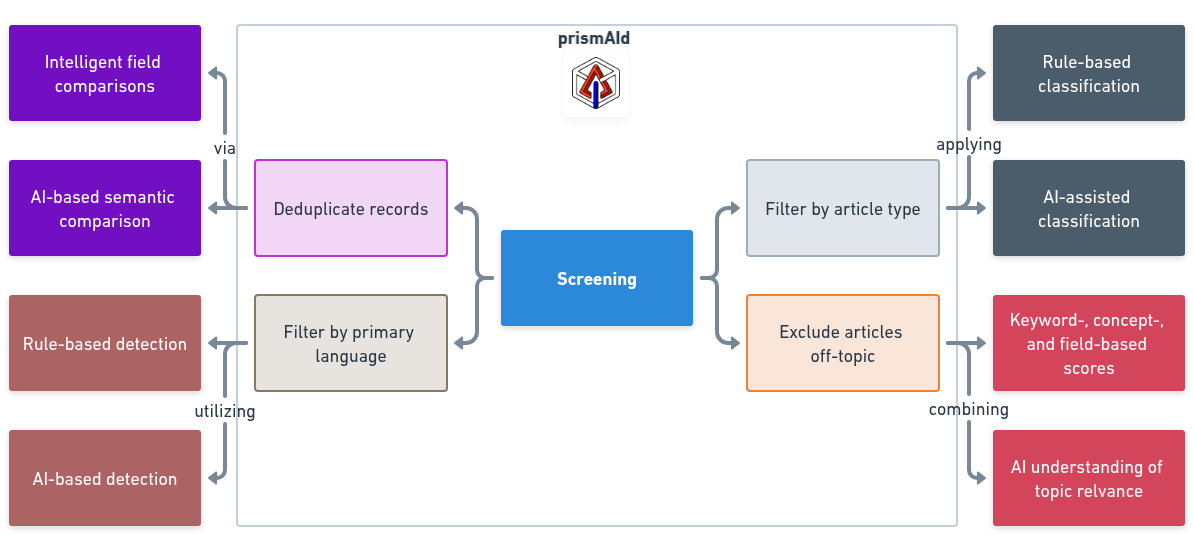
\includegraphics[width=\textwidth]{figures/screening_tools.png}
    \caption{The prismAId Screening tool applies multiple filters in sequence: deduplication, language detection, article type classification, and topic relevance scoring. Each filter can be configured independently to match your systematic review protocol.}
    \label{fig:screening_tools}
\end{figure}

\subsection{Why Screen Before Downloading?}

\begin{itemize}
    \item \textbf{Resource Efficiency}: Avoid downloading and processing irrelevant papers.
    \item \textbf{Time Savings}: Focus manual review efforts on truly relevant literature.
    \item \textbf{Systematic Approach}: Apply consistent inclusion/exclusion criteria across all manuscripts.
    \item \textbf{Audit Trail}: Document exclusion decisions for transparency and reproducibility.
\end{itemize}

\subsection{Preparing Your Screening Configuration}

\begin{configbox}[Configuration: Screening Setup]
\begin{lstlisting}[language=TOML]
# screening_config.toml
[project]
name = "Climate Change Agriculture Screening"
author = "Your Name"
version = "1.0"
input_file = "search_results.csv"  # Export from your database search
output_file = "screening_results"
text_column = "abstract"           # Column containing abstracts
identifier_column = "doi"          # Unique identifier column
output_format = "csv"
log_level = "medium"

[filters.deduplication]
enabled = true
compare_fields = ["title", "doi"]

[filters.language]
enabled = true
accepted_languages = ["en"]

[filters.article_type]
enabled = true
exclude_reviews = true
exclude_editorials = true
exclude_letters = true

[filters.topic_relevance]
enabled = true
topics = ["climate change AND agriculture",
          "crop yield AND temperature"]
min_score = 0.5
\end{lstlisting}
\end{configbox}

\subsection{Running the Screening Tool}

\begin{commandbox}[Command: Screening Manuscripts]
\begin{lstlisting}[language=Bash]
# Run screening on your search results
./prismaid --screening config/screening_config.toml

# Review the screening results
cat results/screening_results.csv | head -n 10
\end{lstlisting}
\end{commandbox}

\tip{Start with conservative filtering settings. You can always apply stricter criteria in a second pass, but you cannot recover manuscripts that were incorrectly excluded.}

\warning{Always manually review a sample of excluded manuscripts to ensure your screening criteria are not too restrictive. Check both included and excluded items for false positives and false negatives.}

\subsection{Understanding Screening Results}

The Screening tool outputs a CSV or JSON file containing:
\begin{itemize}
    \item Original manuscript metadata
    \item Inclusion/exclusion decision
    \item Exclusion reasons (if applicable)
    \item Filter-specific tags (detected language, article type, relevance score)
\end{itemize}

\note{Manuscripts passing all filters will have \texttt{include = true} and can proceed to the download phase. Those excluded will have clear reasons documented for your PRISMA flow diagram.}

\section{Importing and Managing Manuscripts}

Once your project and search are set up, and you've screened your initial results, you'll need to gather and prepare your literature for analysis.

\subsection{Literature Acquisition using the Download Tool}

\subsubsection{Option 1: Downloading from Zotero}\warning{Manuscripts are often protected by copyright. Make sure to respect all applicable rights and use them only within permitted conditions.}
\note{The collection path in Zotero follows a filesystem-like format. For example, "Parent Collection/Sub Collection" or "Group Name/Collection Name" for group libraries.}
\begin{enumerate}
    \item Prepare your Zotero collection with all papers for your systematic review.
    \item Obtain your Zotero user ID and API key.
    \item Create a Zotero configuration file or use command line options.
\end{enumerate}

\begin{configbox}[Configuration: Zotero Download Setup]
\begin{lstlisting}[language=TOML]
# zotero_config.toml
user = "123456789"  # Your Zotero user ID
api_key = "AbCdEfGhIjKlMnOpQrStUv"  # Your Zotero API key
group = "Climate Change Research/Agriculture Papers"  # Your collection path
\end{lstlisting}
\end{configbox}

\begin{commandbox}[Command: Downloading Papers from Zotero]
\begin{lstlisting}[language=Bash]
# Navigate to your project directory
cd my_systematic_review

# Download papers to the papers_pdf directory
./prismaid -download-zotero config/zotero_config.toml -o papers_pdf
\end{lstlisting}
\end{commandbox}

\subsubsection{Option 2: Downloading from URL Lists}
\warning{Some publishers may restrict automatic downloads. Ensure you have appropriate access rights to all papers before attempting to download them.}
\begin{enumerate}
    \item Create a text file with one URL per line for papers you want to download.
    \item Run the URL download command to fetch all papers.
\end{enumerate}

\begin{infobox}[Example URL List File: paper\_urls.txt]
\begin{lstlisting}
https://arxiv.org/pdf/2303.08774.pdf
https://www.science.org/doi/pdf/10.1126/science.1236498
https://www.nature.com/articles/s41586-021-03819-2.pdf
\end{lstlisting}
\end{infobox}

\begin{commandbox}[Command: Downloading Papers from URL List]
\begin{lstlisting}[language=Bash]
# Navigate to your project directory
cd my_systematic_review

# Download papers to the papers_pdf directory
./prismaid -download-URL config/paper_urls.txt -o papers_pdf
\end{lstlisting}
\end{commandbox}



\subsection{Document Conversion using the Convert Tool}

After downloading your papers, you need to convert them to plain text format for analysis.

\begin{commandbox}[Command: Converting PDF Files to Text]
\begin{lstlisting}[language=Bash]
# Navigate to your project directory
cd my_systematic_review

# Convert all PDFs in papers_pdf directory to text files in papers_txt
./prismaid -convert-pdf papers_pdf -o papers_txt
\end{lstlisting}
\end{commandbox}

\reminder{Always manually check a sample of converted files to ensure the conversion quality is acceptable. PDFs with complex layouts or scanned images may not convert perfectly.}
\begin{commandbox}[Command: Converting Multiple File Types]
\begin{lstlisting}[language=Bash]
# For DOCX files
./prismaid -convert-docx papers_docx -o papers_txt

# For HTML files
./prismaid -convert-html papers_html -o papers_txt
\end{lstlisting}
\end{commandbox}

\subsection{Organizing Your Literature Collection}

\begin{enumerate}
    \item Review the converted text files for quality and completeness.\tip{Consider removing unnecessary sections from converted texts, such as references or acknowledgments, to reduce token usage and improve extraction accuracy.}
    \item Remove or fix any problematic conversions.
    \item Optionally, rename files for better organization and tracking.
\end{enumerate}


\subsection{Configure Your Project}

\begin{enumerate}
    \item Generate a basic configuration file using the \texttt{prismAId} initializer.
    \item Customize the configuration file to match your research questions.
\end{enumerate}

You can follow templates and example or create a new project configuration interactively or by using the web-based configurator.

\subsubsection{Interactive Terminal Setup}
\reminder{Always keep a backup of your configuration file before making major modifications.}
\begin{commandbox}[Command: Creating a New Project]
Run the following command:
\begin{lstlisting}[language=Bash]
./prismaid -init
\end{lstlisting}
\end{commandbox}

This prompts you with multiple questions and generates a TOML configuration file.

\subsubsection{Web-Based Setup}

Alternatively, use the web-based configurator available at \href{https://open-and-sustainable.github.io/prismaid/review-configurator.html}{open-and-sustainable.github.io/prismaid/review-configurator.html} to create your configuration file interactively in a browser.

\begin{configbox}[Configuration: Example of Initial Sections of a Configuration]
To configure \texttt{prismAId}, edit the generated \texttt{your\_project.toml} file:
\begin{lstlisting}[language=TOML]
[project]
name = "Use of LLM for systematic review"
author = "John Doe"
version = "1.0"

[project.configuration]
input_directory = "/path/to/txt/files"
results_file_name = "/path/to/save/results"
output_format = "json"
log_level = "low"
duplication = "no"
cot_justification = "no"
summary = "no"
\end{lstlisting}
\end{configbox}
\note{Alternatively, you can use the web-based configurator at \href{https://open-and-sustainable.github.io/prismaid/review-configurator.html}{open-and-sustainable.github.io/prismaid/review-configurator.html} to create your configuration file with a user-friendly interface.}
\begin{commandbox}[Command: Initializing a Project Configuration]
\begin{lstlisting}[language=Bash]
# Navigate to your project directory
cd my_systematic_review

# Initialize a new configuration file
./prismaid -init
\end{lstlisting}
\end{commandbox}

\warning{Always use absolute paths in your configuration file to prevent path-related errors. Relative paths can cause issues when running \texttt{prismAId} from different directories.}
\begin{configbox}[Configuration: Essential Project Settings]
\begin{lstlisting}[language=TOML]
[project]
name = "Effects of Climate Change on Agricultural Yields"
author = "Jane Researcher"
version = "1.0"

[project.configuration]
input_directory = "/home/user/my_systematic_review/papers_txt"
results_file_name = "/home/user/my_systematic_review/results/findings"
output_format = "csv"
log_level = "medium"
duplication = "no"
cot_justification = "yes"
summary = "yes"
\end{lstlisting}
\end{configbox}


\subsection{Configure LLM Settings}

\begin{enumerate}
    \item Obtain API key(s) from your preferred LLM provider(s).\tip{Using a lower temperature setting (0.01-0.1) produces more consistent results, which is generally preferable for systematic reviews where reproducibility is important.}
    \item Set up environment variables or add keys to your configuration file.
    \item Define model settings based on your needs and budget.
\end{enumerate}

\begin{configbox}[Configuration: LLM Provider Setup]
\begin{lstlisting}[language=TOML]
[project.llm.1]
provider = "OpenAI"
api_key = "" # Leave empty to use environment variable
model = "gpt-4o-mini"
temperature = 0.01
tpm_limit = 0
rpm_limit = 0
\end{lstlisting}
\end{configbox}

\section{Running Analyses}

With your literature prepared, you're ready to configure and execute the systematic review.

\begin{figure}[h]
    \centering
    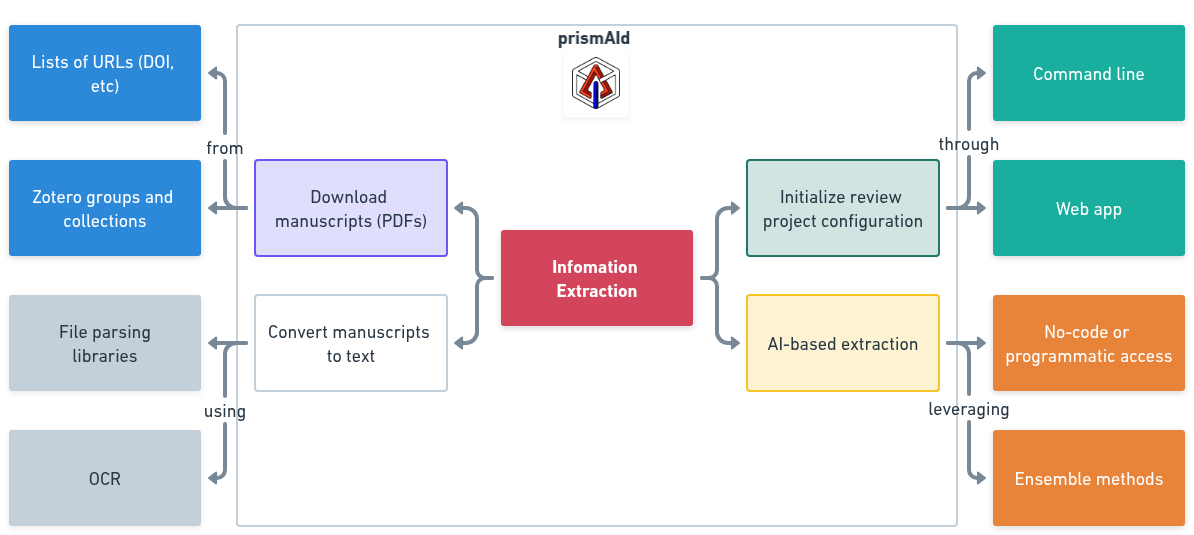
\includegraphics[width=\textwidth]{figures/info_extract_tools.png}
    \caption{The prismAId Review tool processes text documents through configured LLM providers to extract structured information. The tool supports multiple LLM providers, ensemble reviews, and various output formats for comprehensive data extraction.}
    \label{fig:review_tools}
\end{figure}

\subsection{Finalizing Review Configuration}
\tip{When extracting numerical data (like percentages or measurements), use empty value arrays `[""]` to allow the model to extract the exact values rather than categorizing them.}
\begin{enumerate}
    \item Define your prompt structure to instruct the LLM.
    \item Specify the review items (information to extract) in your configuration.
\end{enumerate}

\begin{configbox}[Configuration: Prompt Structure]
\begin{lstlisting}[language=TOML]
[prompt]
persona = "You are an expert agricultural scientist conducting a systematic review on climate change impacts."
task = "Extract specific information about how climate change affects crop yields from the scientific paper text provided."
expected_result = "You should output a JSON object with key findings on crop types, climate factors, and measured impacts."
definitions = "'Crop yield' refers to the quantity of agricultural output harvested per unit of land area."
example = "For example, if the paper states 'wheat yields decreased by 5.2% per degree Celsius increase', report 'wheat' as crop_type, 'temperature increase' as climate_factor, and '-5.2% per °C' as yield_impact."
failsafe = "If information on a specific field is not provided in the document, respond with an empty string value."
\end{lstlisting}
\end{configbox}

\begin{configbox}[Configuration: Review Items Structure]
\begin{lstlisting}[language=TOML]
[review.1]
key = "crop_type"
values = ["wheat", "rice", "maize", "soybean", "barley", "other", "multiple", ""]

[review.2]
key = "climate_factor"
values = ["temperature increase", "precipitation change", "extreme weather", "CO2 levels", "multiple factors", "other", ""]

[review.3]
key = "yield_impact"
values = [""]

[review.4]
key = "adaptation_strategies_discussed"
values = ["yes", "no"]

[review.5]
key = "study_timeframe"
values = ["historical", "current", "future projection", "mixed", ""]
\end{lstlisting}
\end{configbox}

\subsection{Executing the Review}
\note{For large reviews, consider running a test on a small subset of papers first to validate your configuration before processing all documents.}
\begin{commandbox}[Command: Running the Systematic Review]
\begin{lstlisting}[language=Bash]
# Navigate to your project directory
cd my_systematic_review

# Run the review with your configuration file
./prismaid -project config/climate_yield_review.toml
\end{lstlisting}
\end{commandbox}

\subsection{Monitoring Progress}

\begin{enumerate}
    \item Monitor the console output for progress updates.\warning{Long-running reviews may encounter API rate limits. Use the `tpm\_limit` and `rpm\_limit` settings in your configuration to manage API usage and avoid interruptions.}
    \item Check log files if you've enabled detailed logging.
    \item Address any errors or warnings that appear during processing.
\end{enumerate}

\begin{commandbox}[Command: Running with Detailed Logging]
\begin{lstlisting}[language=Bash]
# First modify your config file to set log_level to "high"
# Then run the review
./prismaid -project config/climate_yield_review.toml
\end{lstlisting}
\end{commandbox}

\section{Interpreting Results}

Once your review is complete, you'll need to analyze and understand the extracted information.

\subsection{Understanding Output Files}

\begin{enumerate}
    \item Locate your results file (CSV or JSON format).\reminder{If you enabled `cot\_justification`, each paper will have a corresponding justification file that explains the reasoning behind the extracted information. These can be invaluable for validation and deeper understanding.}
    \item Open supplementary files like justifications or summaries if enabled.
    \item Understand the structure of the output data.
\end{enumerate}

\begin{infobox}[Example CSV Result Structure]
\begin{lstlisting}
filename,crop_type,climate_factor,yield_impact,adaptation_strategies_discussed,study_timeframe
paper1.txt,wheat,temperature increase,-6.4% per °C,yes,future projection
paper2.txt,rice,precipitation change,-3.2% per 10% rainfall decrease,yes,historical
paper3.txt,multiple,multiple factors,varied by region and crop,yes,mixed
\end{lstlisting}
\end{infobox}


\subsection{Validating Extraction Quality}

\begin{enumerate}
    \item Randomly select a subset of papers for manual validation.
    \item Compare the extracted information with the original papers.
    \tip{Aim to manually validate at least 10-20\% of your papers to ensure extraction quality. Focus particularly on papers with unusual or unexpected results.}

    \item Note any discrepancies or patterns in extraction errors.
\end{enumerate}

\subsection{Analyzing Patterns and Trends}

\begin{enumerate}
    \item Import your results into analysis software (R, Python, Excel, etc.).
    \item Perform descriptive statistics on your extracted data.
    \item Identify patterns, relationships, and outliers.
\end{enumerate}

\note{Extracting numerical data from free-text fields like `yield\_impact` may require additional processing before quantitative analysis.}
\begin{commandbox}[Example R Code for Basic Analysis]
\begin{lstlisting}[language=R]
# Load libraries
library(tidyverse)

# Read results
results <- read_csv("results/findings.csv")

# Basic summary
summary(results)

# Count papers by crop type
results %>%
  count(crop_type) %>%
  arrange(desc(n))

# Analyze yield impacts by climate factor
results %>%
  filter(climate_factor %in% c("temperature increase", "precipitation change")) %>%
  group_by(climate_factor, crop_type) %>%
  summarize(n_studies = n()) %>%
  arrange(desc(n_studies))
\end{lstlisting}
\end{commandbox}


\section{Exporting Findings}

The final step is to prepare your findings for presentation, publication, or further analysis.

\subsection{Generating Summary Tables}

\begin{enumerate}
    \item Create summary tables of key findings.
    \item Format the data appropriately for your target audience.\tip{Include both raw data and processed summary tables in your publications to enhance transparency and reproducibility.}
    \item Include relevant metadata about your review process.
\end{enumerate}

\begin{commandbox}[Example Python Code for Table Generation]
\begin{lstlisting}[language=Python]
import pandas as pd
import matplotlib.pyplot as plt

# Load results
results = pd.read_csv("results/findings.csv")

# Create pivot table
pivot = pd.pivot_table(
    results,
    index="crop_type",
    columns="climate_factor",
    values="filename",
    aggfunc="count",
    fill_value=0
)

# Save summary table
pivot.to_csv("results/summary_table.csv")
pivot.to_excel("results/summary_table.xlsx")

# Create visualization
pivot.plot(kind="bar", figsize=(12, 8))
plt.title("Number of Studies by Crop Type and Climate Factor")
plt.tight_layout()
plt.savefig("results/crop_climate_summary.png", dpi=300)
\end{lstlisting}
\end{commandbox}

\subsection{Documenting Your Methodology}

\reminder{For publication, include your full \texttt{prismAId} configuration file (with API keys removed) in supplementary materials to enhance reproducibility.}
\begin{enumerate}
    \item Document your complete review methodology.
    \item Include details about:
    \begin{itemize}
        \item Search strategy and sources
        \item Inclusion/exclusion criteria
        \item \texttt{prismAId} configuration and settings
        \item Validation procedures
        \item Analysis methods
    \end{itemize}
    \item Save your configuration files alongside your results.
\end{enumerate}

\subsection{Visualizing Results}

\warning{Be cautious about drawing causal conclusions from your systematic review findings, especially when AI-assisted tools are used for extraction. Clearly acknowledge limitations in your reporting.}
\begin{enumerate}
    \item Create appropriate visualizations based on your data type.
    \item Consider common visualization types:
    \begin{itemize}
        \item Bar charts for categorical comparisons
        \item Forest plots for effect sizes
        \item Heat maps for multidimensional relationships
        \item Network diagrams for concept relationships
    \end{itemize}
    \item Ensure visualizations accurately represent your findings.
\end{enumerate}

\subsection{Preparing for Publication}

\begin{enumerate}
    \item Format your findings according to journal or conference requirements.
    \item Follow PRISMA or other appropriate reporting guidelines.
    \item Create a PRISMA flow diagram documenting the review process.
    \item Properly cite \texttt{prismAId} in your methodology section.\note{Some journals may have specific requirements or guidelines for reporting AI-assisted analyses. Check with your target journal for any specific policies.}
\end{enumerate}

\begin{infobox}[Example Citation for prismAId]
\begin{lstlisting}
For the systematic information extraction, we used prismAId (Boero, 2024),
an open-source AI-assisted systematic review toolkit. The review was
conducted using [model name] with a temperature setting of [value] and
validation was performed on [percentage]% of the included studies.

Reference:
Boero, R. (2024). prismAId - Open Science AI Tools for Systematic,
Protocol-Based Literature Reviews. Zenodo.
https://doi.org/10.5281/zenodo.11210796
\end{lstlisting}
\end{infobox}

\section{Conclusion}

You have now completed a systematic review using \texttt{prismAId}. By following this step-by-step process, you've:

\begin{itemize}
    \item Set up a structured, reproducible review project
    \item Gathered and prepared literature systematically
    \item Configured and executed an AI-assisted information extraction
    \item Analyzed and validated the extracted information
    \item Prepared your findings for dissemination
\end{itemize}

\reminder{Systematic reviews are iterative processes. Based on your findings, you may decide to refine your research question, adjust your extraction parameters, or expand your literature search. \texttt{prismAId} makes these iterations more efficient than traditional methods.}

The combination of human expertise and AI assistance enables more comprehensive and efficient reviews while maintaining methodological rigor. The next chapter will explore advanced features of \texttt{prismAId} that can further enhance your systematic review capabilities.
